\section{Introduction}
Programming networks to correctly forward flows according to user- and
application-induced policies is difficult and
error-prone~\cite{troubleshooting, bgpmisconfig}. 
At least three
common characteristics of network policies are to blame: (1) A network
may need to satisfy several types of policies, including reachability
(i.e., which end-hosts can communicate), isolation (i.e., which flows
cannot share links), service chaining (i.e., which ``middleboxes'',
e.g., firewalls or load balancers, must be traversed), resilience
(e.g., number of available backup paths), and traffic engineering
(e.g., minimizing average link utilization). (2) The network must
provide certain guarantees in the event of failures. Ideally, every
set of forwarding paths (i.e., data plane) installed in the network
%---either manually or by a control plane---
should conform to these policies, otherwise performance, security, or
availability problems may arise. (3) Most policies are global---i.e.,
they concern end-to-end paths, not individual devices/links.

The global nature of network policies is one motivation for
software-defined networking (SDN). SDN allows paths to be centrally
computed over a global view of the network. However, it is difficult
to ensure forwarding paths are correctly computed and installed in the
presence of failures, even if the SDN controller is
distributed~\cite{hasdn}.

Traditional control planes rely on distributed protocols such as Open
Shortest Path First (OSPF) and Border Gateway Protocol (BGP) to
compute paths; these protocols typically employ variants of least cost
path computation, and react to failures by recomputing least cost
paths and installing forwarding state in routers that induces the
paths. In contrast to centralized SDN, traditional control planes
offer greater fault tolerance; but, determining the appropriate
distributed realization of policies is hard.

Our goal is to {\em automate the process of creating a correct and
  failure-resilient distributed realization of policies in a
  traditional control plane}. We wish to handle a wide range of
policies, e.g., reachability, service chaining, and traffic
engineering, to meet applications' diverse security and compliance
requirements.  With increasing sizes of networks, we must further
provide support for realizing hierarchical control planes (where a
network is split into several domains atop which a hierarchy of
control plane configurations is deployed) to ensure scalability,
necessitating the use of multiple intra- and inter-domain routing
protocols (e.g., OSPF and BGP).  Finally, and most importantly, we
want configurations that are resilient to network malfunctions such as
link failures.  Thus, our work contrasts with prior
efforts~\cite{netegg, propane, merlin, simple, fattire, netkat,
  netkatcompiler, sol}, which generate SDN- or BGP-specific control
planes for a limited range of policies (e.g., peering) 
and/or do not attempt to be resilient to failures.



The problem of synthesizing router configurations
for which the distributed control plane is
resilient to failures and it
generates policy-compliant paths 
is computationally hard. 
First, even generating a set of policy-compliant 
paths for an SDN  is 
computationally hard---e.g., enforcing isolated
paths is NP-complete. 
Second, to infer the concrete
set of paths induced by network configurations, 
one has to incorporate
into synthesis
complex concepts---e.g., reasoning about shortest path algorithms
requires constraints in complex
theories that combine propositional logic (SAT) 
with linear rational
arithmetic (LRA). Even with recent 
advances in Satisfiability Modulo Theories
(SMT) solvers, 
approaches that directly generate configurations  from policies
do not scale to
even moderately-sized networks or 
sets of policies~\cite{synet}.
Third, to generate resilient control planes one has to reason
about how different protocols react to failures, 
which further complicates an already intractable synthesis
problem. 

\begin{wrapfigure}{r}{0.4\columnwidth}
	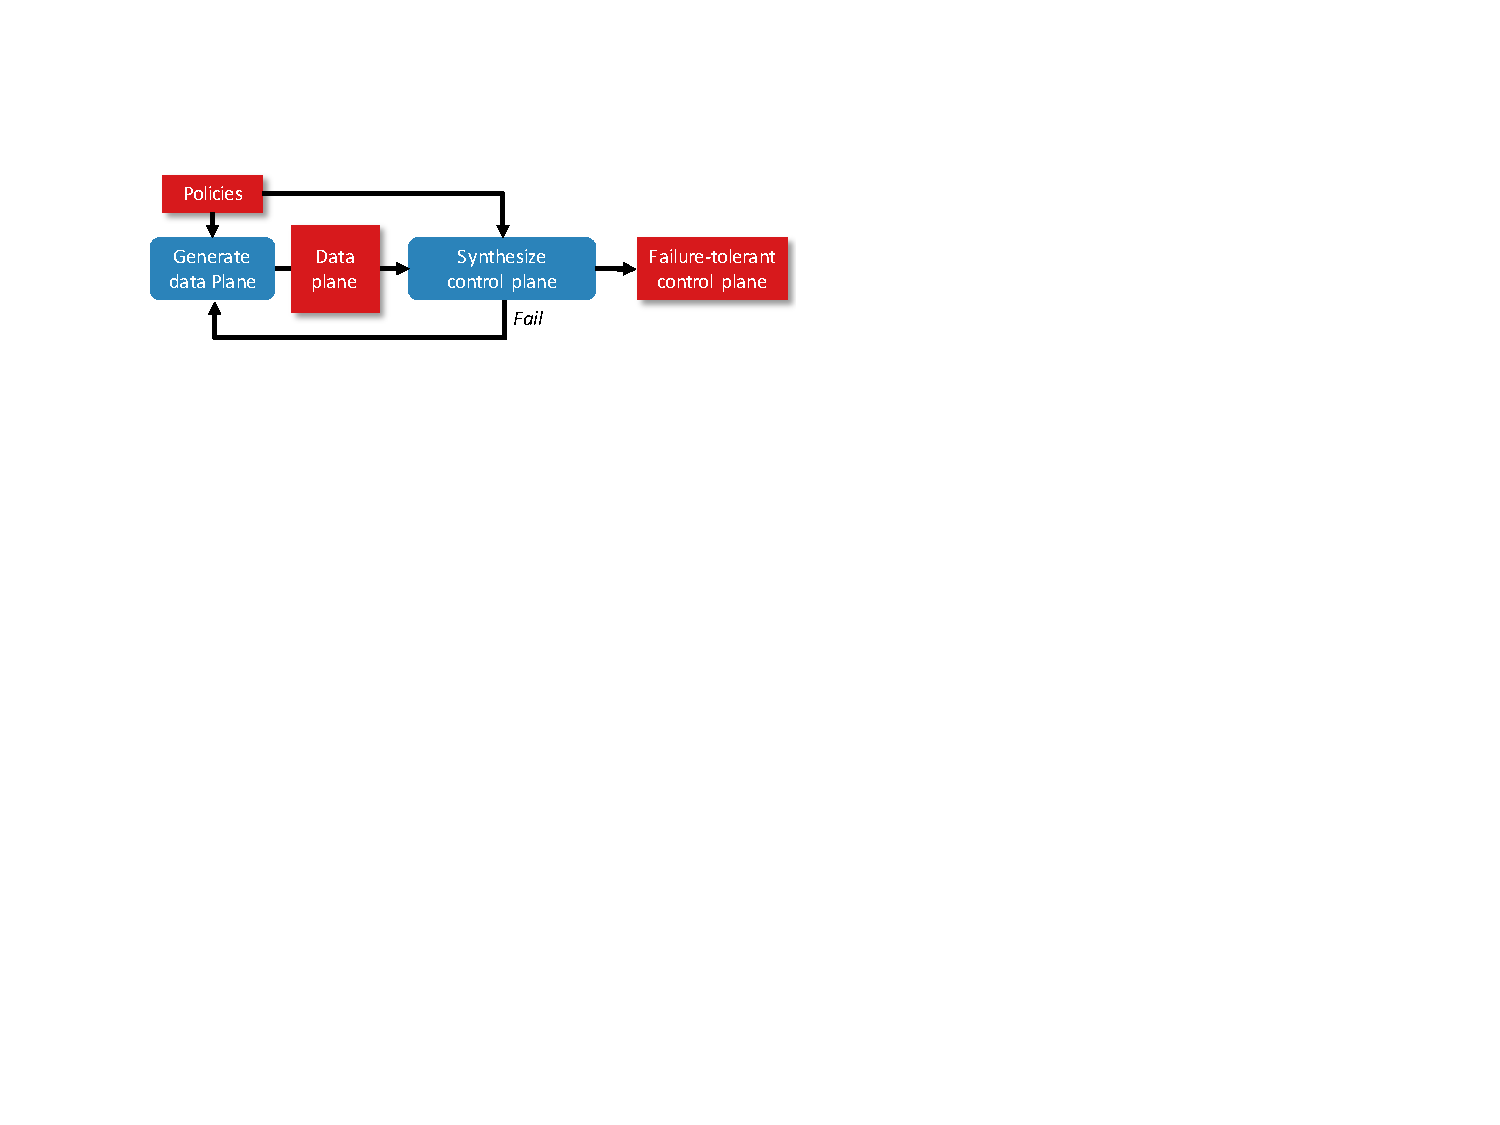
\includegraphics[width=\linewidth]{figures/architecture.pdf}
	\compactcaption{Two-phase process for generating a control plane
		with failure-tolerance properties}
	\label{fig:architecture}
\end{wrapfigure}

In this paper, we present \name, a new approach for synthesizing
highly resilient policy-compliant configurations.
Unlike previous approaches, \name uses a two-phased approach 
(\Cref{fig:architecture}) 
that does not attempt to generate 
a policy-compliant control plane in a single step.
First, \name 
uses \genesis~\cite{genesis}
to synthesize paths---i.e., the network forwarding state---that are compliant
with given policies, such as, waypoint, isolation,
and traffic engineering.
\name generates 
intra-domain (shortest-path OSPF) and inter-domain (BGP) router configurations
that induce the forwarding
state synthesized by \genesis and provide high resilience. 
%We consider hierarchical networks  routers run
%OSPF for intra-domain routing, while domains use BGP for inter-domain
%routing. Moreover, routers can install static routes---i.e., default routes that can bypass the other two protocols.

We investigate three different settings with different policies and resilience requirements
and show how \name, using its two-phase approach, can effectively generate
highly-resilient and policy-compliant solutions.

First, we consider a setting in which the operator of a hierarchically
structured network wants to enforce a large diverse set of complex
policies (waypoint-compliance, isolation, traffic engineering, etc).
The operator also requires a simple notion of
\emph{connectivity-resilience} to guarantee that, under most common
link failures, packets can still reach their destination.
%In general, in the absence of static routes a network can support
%a number of link failures equal to the min-cut of the network, regardless
%of the OSPF and BGP configurations.
%However, we might need static routes to generate policy-compliant configurations.
%Static routes can cause unexpected network behaviors after a failure---e.g., a forwarding loop---and
%we argue that the \emph{connectivity-resilience} of a configuration is related to the its number of static routes.
To increase connectivity-resilience, \name tries to produce
policy-compliant configurations with a small number of {\em static
  routes}---i.e., static router configurations where routers have
fixed next hops for a destination that bypass routes computed by routing protocols (OSPF and BGP).
%---helps 
%increasing \emph{connectivity-resilience} and
%decreasing configuration complexity. 
%thus, easing automated
%verification~\cite{batfish, arc, era} and improving readability for
%performing future manual changes.
%Therefore, \name aims at producing policy-compliant configurations with a small number of static routes.
To do so, \name synthesizes OSPF configurations using linear constraint solving to compute
link weights and uses the unsatisfiable cores
of failed solving attempts to learn when to introduce static routes.
\name synthesizes BGP configurations directly from the domain mapping (i.e., which router belongs to what domain) and the paths.
Using these techniques, \name can generate configurations that are
$11\%$ more resilient than configurations that only static static routes.

Second, we consider a setting in which the operator wants to enforce a
set of policies and wants to guarantee that, for most of the common
link failures, the resulting configuration is still policy-compliant.
We call this notion \emph{policy-resilience}.  Given the complexity of
this problem, we focus on a {\rm restricted class} of policies.  In
particular, for each class of packets, we allow the operator to
specify a set of waypoints---e.g., a set of firewalls---that packets
must traverse before reaching their destination.  To generate
configurations with high policy-resilience we modify our linear
constraints to guarantee that at least two paths that traverse the
waypoints have path cost (e.g., OSPF path cost) than any path not
going through a waypoint.  Using this improved technique, \name can
generate configurations that are $140\%$ more policy-resilient than
configurations generated with our first technique.


Finally, we consider a setting in which the operator has the
flexibility to assign routers to different domains.  We present a
stochastic search technique that uses this flexibility to look for
ways to assign routers to different domains so that the synthesized
configurations have higher resilience.  Using this search technique,
\name can further improve the resilience of the configurations
generated by the previous two techniques by $10\%$.

%We evaluate \name on medium-sized topologies and show that
%\name can synthesize OSPF configurations for 200 paths in 200
%seconds for a 40 node ISP topology, and achieve greater than 
%50\% resilience for fat-tree topologies.
%\todo{what does resilient mean here? this last para and contrib need to be rewritten
%after eval}
% On average, using MCMC, \name can increase
%endpoint resilience by $1.6\times$ and 
%reduce configuration overhead
%by $0.3\times$
%for a 125-node ISP topology.


%% Automatically synthesizing distributed realizations 
%% of network policies is an
%% important step towards simplifying 
%% network management and providing an 
%% SDN-like interface for programming networks 
%% running distributed routing protocols. 
%% Our approach is an important
%% contribution towards the vision of 
%% intent-driven networking~\cite{intent}.

\paragraph{Contributions} We make the following contributions.
\begin{itemize}	
    \item \name, a framework for
	that enforces policies in `traditional' (OSPF and BGP) networks
	by synthesizing highly-resilient router configurations. 		
	\name differs from existing approaches in that it uses concrete
	paths to guide the synthesis search instead of directly generating policy-compliant
	configurations.

	\item An algorithm for synthesizing policy-compliant
          configurations with few statically assigned routes. This
          algorithm yields configurations with high network
          connectivity even in the presence of link failures
          (\S~\ref{sec:config-synthesis}).

	\item An algorithm for synthesizing policy-compliant 		
		 configurations that is specialized for waypoint policies. 
		 This algorithm yields configurations that have
		 high policy compliance even in the presence of link failures (\S~\ref{sec:ospfwaypoint}). 
	
	\item A stochastic search mechanism for finding 
		partitions of the network into multiple routing domains which
		yield configurations with higher resilience (\S~\ref{sec:synth-dom-ass}).
	
	\item An implementation of \name
	together with an evaluation of its synthesis algorithms
	 for different topologies and workloads. 
	 Our results show that \name can produce highly resilient and policy compliant
	 network configurations (\S~\ref{sec:evaluation}). 
\end{itemize}
